\part{Machine Learning}

\section{Probabilities}

\subsection{Binary variables}

\subsubsection{Bernoulli distribution}

Suppose $x = \{0, 1\}$ is a binary random variable and the probability of $x = 1$ is denoted $\mu$.
\begin{equation}
    \mathcal{P}(x=1|\mu) = \mu
\end{equation}

$x$ follows the Bernoulli distribution defined as
\begin{equation}
    Bern(x|\mu) = \mu^x (1-\mu)^{1-x}
\end{equation}
It can be easily shown that its expectation and variance are
\begin{equation}
    \mathbb{E}[x] = \mu
\end{equation}
\begin{equation}
    var[x] = \mu(1-\mu)
\end{equation}

Now suppose we have a set of observations of $x$, $D = \{x_1, x_2, \dots x_N\}$. We can construct the likelihood function
\begin{equation}
    p(\mathcal{D}|\mu) = \prod_{i=1}^{N} p(x_i|\mu) = \prod_{i=1}^{N} \mu^{x_i} (1-\mu)^{1-x_i}
\end{equation}

With a statistical approach it is possible to estimate the value of $\mu$ by maximizing the likelihood function, or equivalently, maximizing the \textit{log likelihood} function.
\begin{equation}
    \ln{p(\mathcal{D}|\mu)}=\sum_{i=1}^{N} \ln{p(x_i|\mu)} = \sum_{i=1}^{N} \{x_i \ln{\mu} + (1-x_i) \ln{(1-\mu)}\}
\end{equation}

I we set the derivative of $\ln{p(\mathcal{D}|\mu)}$ with respect to $\mu$ to zero, we get 
\begin{equation}
    \mu_{ML} = \frac{1}{N}\sum_{i=1}^N x_i
\end{equation}
In other words, this is the number of one divided by the total number of experiences.
Now suppose, we flip a coin 3 times and get 3 times 1. The maximum likelihood is $\mu = 1$. Common sense tells us that it seems unreasonable and we will see that we need to use priors (on the distribution of $\mu$ for example) to solve the problem.

\subsubsection{Binomial distribution}
Now suppose that we want to know the number of times $m$ that $x=1$ among $N$ experiences. This follows a binomial distribution given by
\begin{equation}
    Bin(m|\mu, N) = \left(\begin{array}{c}
        N \\ m
    \end{array}\right)
    \mu^{m} (1-\mu)^{N-m}
\end{equation}

Its expectation and variance are given by
\begin{equation}
    \mathbb{E}[m] = N\mu
\end{equation}
\begin{equation}
    var[m] = N\mu(1-\mu)
\end{equation}

\subsubsection{Multinomial distribution}
We often encounter discrete variables which can take one of $K$ mutually exclusive states. We represent it with a K-dimensional vector where each element can be 1 or 0. $x = (0, 0, 1, 0, 0, 0)^T$. We denote the probability if $x_k=1$ by $\mu_k$. Then, the distribution of $x$ is given by
\begin{equation}
    p(x|\mu) = \prod_{k=1}^{K} \mu_k^{x_k}
\end{equation}
where $\mu=(\mu_1, \dots, \mu_K)$ and the parameters $\mu_k$ are constrained by $\mu_k \ge 0$ and $\sum_{k=1}^K \mu_k = 1$.

\subsection{Gaussian distribution}
For a N-dimensional random vector $x$, the multivariate Gaussian distribution is given by
\begin{equation}
    \mathcal{N}(x|\mu,\Sigma^2) = \frac{1}{(2\pi)^{D/2}\sqrt{|\Sigma|}} \exp\{-\frac{1}{2}(x-\mu)^T \Sigma^{-1}(x-\mu)\}
\end{equation}
The Gaussian distribution arises in many contexts. For example, the Gaussian distribution is the distribution which maximizes the \textit{entropy}.
Also, the \textit{central limit theorem} tells us that the sum of a set of random variables tends to follow a Gaussian distribution.

The covariance matrix $\Sigma$ is symmetric and have real eigen values and its eigen vectors can be chosen to form an orthonormal set.
\begin{equation}
    \Sigma u_i = \lambda_i u_i
\end{equation}
$\Sigma$ can be decomposed in $\Sigma = U S U^T$, where $U$ has the eigen vectors as columns and $S$ is a diagonal matrix. This implies that $\Sigma^{-1} = (USU^T)^{-1} = U S^{-1} U^T$. We can then use a change of variable $y = U^T(x-\mu)$
\begin{equation}
    (x-\mu)^T \Sigma^{-1} (x-\mu) = y^T S^{-1} y
\end{equation}
In this new coordinate system, the Gaussian distribution becomes a set of N independent 1-dimensional Gaussian distributions. 

One limitation of Gaussian distribution is the large number of free parameters. Considering a D-dimensional Gaussian distribution, its covariance matrix will have $D(D+1)/2$ independent parameters and another $D$ parameters for $\mu$. This means the number of parameters grows quadratically with the dimension.
One way of addressing that is to add constraints on the form of the covariance matrix. We could restrict it to be diagonal for example ($\Sigma=diag(\sigma_i^2)$). This give $2\times D$ parameters. We could even further restrict it to $\Sigma = \sigma^2 I$. This is called an \textit{Isotropic Gaussian distribution}.

Another limitation is that a Gaussian distribution is intrinsically uniquely modal (i.e it has a single maximum) and thus is unable to provide a good approximation to multimodal distributions.

\paragraph{Conditional Gaussian distributions}
An important property of multivariate Gaussian distribution is that if two sets of variables are jointly Gaussian, then the conditional distribution of one set conditioned on the other is also Gaussian. Similarly, the \textbf{marginal distribution} of either set is also Gaussian.

\paragraph{Precision matrix}
The \textit{precision matrix} is defined as the inverse of the covariance matrix.
\begin{equation}
    \Lambda = \Sigma^{-1}
\end{equation}

\subsubsection{Maximum Likelihood for Gaussian distribution}
Given a dataset $X = (x_1, x_2, \dots, x_n)^T$, in which the observations are assumed to be drawn independently from a multivariate Gaussian distribution, it is possible to estimate the parameters of this Gaussian distribution by maximizing the likelihood (or equivalently the log-likelihood) function.

\begin{equation}
    \ln{p(X|\mu, \Sigma)} = -\frac{ND}{2}\ln{(2\pi)}-\frac{N}{2}\ln{|\Sigma|}-\frac{1}{2}\sum_{n=1}^{N} (x_n - \mu)^T \Sigma^{-1} (x_n - \mu)
\end{equation}
We can compute the derivative of the likelihood function.
\begin{equation}
    \frac{\delta}{\delta \mu} \ln{p(X|\mu, \Sigma)} = \sum_{n=1}^{N} \Sigma^{-1} (x_n - \mu)
\end{equation}

By setting the derivative to zero, we can find the maximum likelihood estimate of $\mu$ and $\Sigma$.
\begin{equation}
    \mu_ {ML} = \frac{1}{N}\sum_{n=1}^{N} x_n
\end{equation}
\begin{equation}
    \Sigma_{ML} = \frac{1}{N} \sum_{n=1}^{N} (x_n - \mu_{ML})(x_n - \mu_{ML})^T
\end{equation}

\underline{Warning:} We can compute the expectation for the maximum likelihood estimate of the mean and covariance. We will obtain:
\begin{equation}
    \mathbb{E}[\mu_ {ML}] = \mu
\end{equation}
\begin{equation}
    \mathbb{E}[\Sigma_{ML}] = \frac{N-1}{N}\Sigma
\end{equation}

The maximum likelihood estimate of the covariance has an expectation lower than the true covariance and hence it is biased. We can correct this bias by using another estimator.
An intuition for this bias is that $\mathbb{E}[\mu_{ML}^2]$ is biased compared to $\mu^2$. When we over- under-estimate the mean, the error compensate but the square causes the error to be always positive and thus biased.

\subsubsection{Sequential estimation}
When the dataset is too large or for online processing, it can be very useful to do sequential estimation. For example, it is possible to compute the influence of the last observation in the Maximum Likelihood of the mean.
\begin{equation}
\begin{split}
    \mu_{ML}^{(N)} & = \frac{1}{N}\sum_{n=1}^{N} x_n \\
     & = \frac{1}{N} x_n + \frac{1}{N}\sum_{x=1}^{N-1} x_n \\
     & = \frac{1}{N}x_n + \frac{N-1}{N}\mu_{ML}^{(N-1)} \\
     & =\mu_{ML}^{(N-1)} + \frac{1}{N}(x_n - \mu_{ML}^{(N-1)})
\end{split}
\end{equation}

This show that the last observation has an influence proportional to the current $N$. It tries to draw the mean towards itself, but, because of the proportional factor, each new data has less and less impact as the number of observations increases.

\subsubsection{Bayesian inference for the Gaussian}

The maximum likelihood framework gives estimate of the parameters $\mu$ and $\Sigma$. Here we develop a Bayesian treatment by introduction priors distributions over these parameters.

\underline{Example}: Estimating the mean of a Gaussian random variable knowing its variance $\sigma^2$. The likelihood function, that is the probability of the observed data $\boldsymbol{X}$ given $\mu$ is given by

\begin{equation}
    p(\boldsymbol{X}|\mu) = \prod_{n=1}^{N} p(x_n | \mu) = \frac{1}{(2\pi \sigma^2)^{N/2}} exp\left[ -\frac{1}{2\sigma^2}\sum_{n=1}^{N} (x_n - \mu)^2 \right]
\end{equation}
\underline{Note}: The likelihood function $p(\boldsymbol{X}|\mu)$ is not a probability distribution over $\mu$ and is not normalized.

We see that the likelihood function takes the form of the exponential of a quadratic form in $\mu$. Thus, if we choose a prior $p(\mu)$ given by a Gaussian, it will be a conjugate distribution for this likelihood function because the corresponding posterior will be a product of two exponentials of quadratic functions of $\mu$ and hence will also be Gaussian.
We take our prior distribution of $\mu$ as
\begin{equation}
    p(\mu) = \mathcal{N}(\mu|\mu_0, \sigma_0^2)
\end{equation}
The posterior distribution is given by 
\begin{equation}
    p(\mu|\boldsymbol{X}) \propto p(\boldsymbol{X}|\mu) p(\mu)
\end{equation}

Simple manipulation show that the posterior distribution is given by

\begin{equation}
    p(\mu | \boldsymbol{X}) = \mathcal{N}(\mu | \mu_N, \sigma_N^2)
\end{equation}
where
\begin{equation}
    \mu_N = \frac{\sigma^2}{N\sigma_0^2 + \sigma^2} \mu_0 + \frac{N\sigma_0^2}{N\sigma_0^2 + \sigma^2}\mu_{ML}
\end{equation}
\begin{equation}
    \frac{1}{\sigma_N^2} = \frac{1}{\sigma_0^2} + \frac{N}{\sigma^2}
\end{equation}

where $\mu_{ML}$ is the maximum likelihood solution for $\mu$ given by the samples mean
\begin{equation}
    \mu_{ML} = \frac{1}{N}\sum_{n=1}^{N} x_n
\end{equation}

It is important to note a few things:
\begin{itemize}
    \item The mean of the posterior distribution is a compromise between the prior mean $\mu_0$ and the maximum likelihood solution $\mu_{ML}$.
    \item If the number of observations is $N = 0$, the posterior mean is the prior mean $\mu_0^2$.
    \item If $N \rightarrow \infty$ the posterior mean is the maximum likelihood solution $\mu_{ML}$.
    \item For the variance of the posterior distribution, it is easier to look at its inverse (the precision).
    \item The precisions are additive. Thus the precision of the posterior is the precision of the prior plus a contribution of the data precision for each observed data point.
    \item If $N = 0$, the posterior variance is equal to the prior variance.
    \item If $N \rightarrow \infty$, the posterior variance $\sigma_N^2$ goes to zero and the posterior distribution becomes infinitely peaked around the maximum likelihood solution.
    \item For a finite number of observations $N$, if we take a prior variance very large $\sigma_0^2 \rightarrow \infty$, the posterior mean reduces to the maximum likelihood and the posterior variance reduces to $\sigma_N^2 = \sigma^2/N$.
\end{itemize}

\subsection{Dirichlet distribution}

The Dirichlet distribution is a \textbf{continuous multivariate} probability distribution. It is the \textbf{multivariate generalization} of the \textbf{Beta} distribution.

Its support is the set of K-dimensional vectors $x$ with $x_i \in [0, 1]$ and $\norm{x} = 1$. In other words, its is a categorical distribution over the probability simplex.
This support can also be seen as a probability distribution. This means we can imagine that the Dirichlet gives a distribution over probabilities.

\noindent\makebox[\linewidth]{\rule{\paperwidth}{0.4pt}}
\paragraph{Note on simplex}
\begin{itemize}
    \item For $K=2$, the unit simplex is the triangle formed by $(0, 0), (1, 0), (0, 1)$ and the probability simplex is the line from $(1, 0)$ to $(0, 1)$.
    \item For $K=3$, the unit simplex is the tetrahedron formed by $(0, 0, 0), (1, 0, 0), (0, 1, 0), (0, 0, 1)$ and the probability simplex is the triangular face between $(1, 0, 0), (0, 1, 0), (0, 0, 1)$.
\end{itemize}
\noindent\makebox[\linewidth]{\rule{\paperwidth}{0.4pt}}


A Dirichlet distribution has a K-dimensional vector $\alpha$ of non-negative numbers as parameter. The probability of a K-dimensional vector is given by


\begin{equation}
    Dir(\mu|\alpha) = \frac{\Gamma(\alpha_0)}{\Gamma(\alpha_1) \hdots \Gamma(\alpha_K)} \prod_{k=1}^K \mu_k^{\alpha_k-1}
\end{equation}


where $\Gamma(x)$ is the Gamma functions and $\alpha_0 = \sum_{k=1}^K \alpha_k$.

\begin{equation}
    E[\mu_i] = \frac{\alpha_i}{\alpha_0}
\end{equation}
\begin{equation}
    Mode[\mu] = \left( \frac{\alpha_1-1}{\alpha_0-n}, \dots, \frac{\alpha_i-1}{\alpha_0-n},  \dots, \frac{\alpha_n-1}{\alpha_0-n}  \right)
\end{equation}
\begin{equation}
    Var[\mu_i] = \frac{\alpha_i(\alpha_0-\alpha_i)}{\alpha_0^2(\alpha_0+1)}
\end{equation}

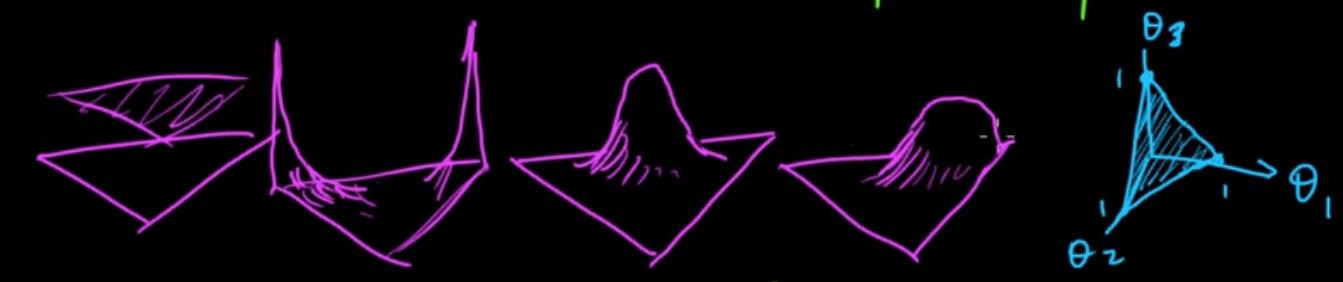
\includegraphics[scale=0.25]{content/Dirichlet_distribution.png}


If we ignore the normalization factor, we ca see the the parameters $\alpha_i$ controls the distribution. In particular:
\begin{itemize}
    \item if $\alpha_i = 1$, all $\mu_k^{\alpha_k-1}$ will be $1$ and thus the distribution is \textbf{uniform}.
    \item if some $\alpha_i$ becomes large, they will create some bumps (like on the 4th image)
    \item if some $\alpha_i$ becomes small (less than 1 and tend to 0), the probability will go to infinity (this is because all $\mu_k \in [0, 1]$ (like on the 2nd image).
\end{itemize}


The Dirichlet distribution is linked to the multinomial one, the same way the Beta distribution is linked to the binomiale one.

\subsection{Laplace distribution}
A Laplace distribution is a continuous probability distribution.
A random variable has a $Laplace(\mu, b)$ distribution if its probability density function is

\begin{equation}
    f(x|\mu, b) = \frac{1}{2b}exp^{-\frac{|x-\mu|}{b}}
\end{equation}

\begin{equation}
    E[x] = \mu
\end{equation}
\begin{equation}
    Var[x] = 2b^2
\end{equation}

\subsection{Link between regularization and prior distributions}
The notion of regularization can be illustrated by a very simple example of linear regression. It consists of shrinking (l2), or even zeroing (l1), some of the parameters.

\paragraph{Equivalence}
Optimizing model weights to minimize a squared error loss function with L2 regularization is equivalent to finding the weights that are the most likely under a posterior distribution evaluated using Bayes rule, with a zero-mean independent Gaussian weights prior.

\begin{equation}
L = \underbrace{\sum_{n=1}^N (\mathbf{y}^{(n)}-f_\mathbf{w}(\mathbf{x}^{(n)}))^2}_{original\;L2\;function} \;+ \underbrace{\lambda \sum_{i=1}^{K} w_i^2}_{regularization}
\end{equation}

Recall the multivariate Gaussian distribution is
\begin{equation}
    \mathcal{N}(\mathbf{x}; \mu, \Sigma) = \frac{1}{(2\pi)^{D/2} |\Sigma|^{1/2}} e^{\left(-\frac{1}{2} (\mathbf{x}-\mu)^T \Sigma^{-1}(\mathbf{x}-\mu)\right)}
\end{equation}

Using Bayes rule, we have $posterior \propto likelihood \times prior$.
\begin{align}
    p(\mathbf{w}|\mathcal{D}) & \propto p(\mathcal{D}|\mathbf{w}) p(\mathbf{w}) \\
     & \propto \prod_n^N \mathcal{N}(y^{(n)}; f_\mathbf{w}(\mathbf{x}^{(n)}), \sigma_y^2) \prod_{i=1}^K \mathcal{N}(\mathbf{w}; 0, \sigma_\mathbf{w}^2)
\end{align}

The left part of the equation is the \textbf{likelihood} of observing the data. It has the form of a product of Gaussian because we assumed an additional zero-mean independent Gaussian noise on our observations.

The right part is the \textbf{prior} distribution of our weights (or parameters). This is a multivariate zero-mean uncorrelated Gaussian. Because the weights are independent, it is possible to write it as a product.

If we take the negative log-probability, we get
\begin{align}
    -\log[p(\mathbf{w}|\mathcal{D})] & = -\sum_ {n=1}^{N} \log[\mathcal{N}(y^{(n)}; f_{\mathbf{w}}(\mathbf{x}^{(n)}), \sigma_y^2)] - \sum_{i=1}^K \log[\mathcal{N}(w_i; 0, \sigma_{\mathbf{w}}^2)] + const \\
    & = \frac{1}{2\sigma_y^2} \sum_{n=1}^N (y^{(n)} - f_{\mathbf{w}}(\mathbf{x}^{(n)}))^2 + \frac{1}{2\sigma_{\mathbf{w}}^2} \sum_{i=1}^K w_i^2 + const
\end{align}

We can ignore the constant and the scale factors, because they do not change the location of the minima (the constant does nothing and the multiplicator just scales the learning rate)
We can easily see that the negative log-posterior probability is equivalent to the squared-error loss function with L2 regularization.

\paragraph{L1 Regularization}
Similarly, it can be shown that a L1 regularization term is equivalent to a \textit{Laplace} prior distribution on the weights.



\section{Data Science questions}

\subsection{Central Limit Theorem}
In some situations, when \textbf{independent random variables} are added, their \textbf{properly normalized sum} tends toward a \textbf{normal distribution}, even if the original variables themselves were not normally distributed.

\subsection{Sampling}
Sampling is a statistical analysis technique used to select a subset of data points in a dataset in order to identify patterns and trends.

\subsection{Selection bias}
Selection bias (or Sampling bias) occurs when the sample data used for modeling has characteristics that are not representative of the future population that the model will see. That is when a subsets of data are systematically (i.e not randomly) excluded from analysis.

\subsection{Bernoulli, Binomial, Geometric, Poisson}
All these distributions are for discrete random variables.

\paragraph{A Bernoulli distribution} models a single experiment that can take 2 outcomes 0 or 1, with the associated probabilities $p$ and $1-p$.

\paragraph{A Binomial distribution} models the number of successes when N independent Bernoulli's experiments are done successively. 

\paragraph{A Geometric distribution} models the number of independent Bernoulli's experiments needed until the first success.

\paragraph{A Poisson distribution} models the number of occurrences of events happening in a time interval, if these events happen with a known mean frequency and independently from the elapsed time since the last occurrence.

